\documentclass[journal,12pt,twocolumn]{IEEEtran}
%
\usepackage{setspace}
\usepackage{gensymb}
\usepackage{xcolor}
\usepackage{caption}
\usepackage{polynom}
%\usepackage{subcaption}
%\doublespacing
\singlespacing

%\usepackage{graphicx}
%\usepackage{amssymb}
%\usepackage{relsize}
\usepackage[cmex10]{amsmath}
\usepackage{mathtools}
%\usepackage{amsthm}
%\interdisplaylinepenalty=2500
%\savesymbol{iint}
%\usepackage{txfonts}
%\restoresymbol{TXF}{iint}
%\usepackage{wasysym}
\usepackage{hyperref}
\usepackage{amsthm}
\usepackage{mathrsfs}
\usepackage{txfonts}
\usepackage{stfloats}
\usepackage{cite}
\usepackage{cases}
\usepackage{subfig}
%\usepackage{xtab}
\usepackage{longtable}
\usepackage{multirow}
%\usepackage{algorithm}
%\usepackage{algpseudocode}
%\usepackage{enumerate}
\usepackage{enumitem}
\usepackage{mathtools}
%\usepackage{iithtlc}
%\usepackage[framemethod=tikz]{mdframed}
\usepackage{listings}


%\usepackage{stmaryrd}


%\usepackage{wasysym}
%\newcounter{MYtempeqncnt}
\DeclareMathOperator*{\Res}{Res}
%\renewcommand{\baselinestretch}{2}
\renewcommand\thesection{\arabic{section}}
\renewcommand\thesubsection{\thesection.\arabic{subsection}}
\renewcommand\thesubsubsection{\thesubsection.\arabic{subsubsection}}

\renewcommand\thesectiondis{\arabic{section}}
\renewcommand\thesubsectiondis{\thesectiondis.\arabic{subsection}}
\renewcommand\thesubsubsectiondis{\thesubsectiondis.\arabic{subsubsection}}

%\renewcommand{\labelenumi}{\textbf{\theenumi}}
%\renewcommand{\theenumi}{P.\arabic{enumi}}

% correct bad hyphenation here
\hyphenation{op-tical net-works semi-conduc-tor}

\lstset{
language=Python,
frame=single, 
breaklines=true,
columns=fullflexible
}



\begin{document}
%

\theoremstyle{definition}
\newtheorem{theorem}{Theorem}[section]
\newtheorem{problem}{Problem}
\newtheorem{proposition}{Proposition}[section]
\newtheorem{lemma}{Lemma}[section]
\newtheorem{corollary}[theorem]{Corollary}
\newtheorem{example}{Example}[section]
\newtheorem{definition}{Definition}[section]
%\newtheorem{algorithm}{Algorithm}[section]
%\newtheorem{cor}{Corollary}
\newcommand{\BEQA}{\begin{eqnarray}}
\newcommand{\EEQA}{\end{eqnarray}}
\newcommand{\define}{\stackrel{\triangle}{=}}

\bibliographystyle{IEEEtran}
%\bibliographystyle{ieeetr}

\providecommand{\nCr}[2]{\,^{#1}C_{#2}} % nCr
\providecommand{\nPr}[2]{\,^{#1}P_{#2}} % nPr
\providecommand{\mbf}{\mathbf}
\providecommand{\pr}[1]{\ensuremath{\Pr\left(#1\right)}}
\providecommand{\qfunc}[1]{\ensuremath{Q\left(#1\right)}}
\providecommand{\sbrak}[1]{\ensuremath{{}\left[#1\right]}}
\providecommand{\lsbrak}[1]{\ensuremath{{}\left[#1\right.}}
\providecommand{\rsbrak}[1]{\ensuremath{{}\left.#1\right]}}
\providecommand{\brak}[1]{\ensuremath{\left(#1\right)}}
\providecommand{\lbrak}[1]{\ensuremath{\left(#1\right.}}
\providecommand{\rbrak}[1]{\ensuremath{\left.#1\right)}}
\providecommand{\cbrak}[1]{\ensuremath{\left\{#1\right\}}}
\providecommand{\lcbrak}[1]{\ensuremath{\left\{#1\right.}}
\providecommand{\rcbrak}[1]{\ensuremath{\left.#1\right\}}}
\theoremstyle{remark}
\newtheorem{rem}{Remark}
\newcommand{\sgn}{\mathop{\mathrm{sgn}}}
\newcommand{\myvec}[1]{\ensuremath{\begin{pmatrix}#1\end{pmatrix}}}
\newcommand{\mybvec}[1]{\ensuremath{\begin{bmatrix}#1\end{bmatrix}}}
\newcommand{\w}[2]{\ensuremath{W_{#1}^{#2}}}
\providecommand{\abs}[1]{\left\vert#1\right\vert}
\providecommand{\res}[1]{\Res\displaylimits_{#1}} 
\providecommand{\norm}[1]{\lVert#1\rVert}
\providecommand{\mtx}[1]{\mathbf{#1}}
\providecommand{\mean}[1]{E\left[ #1 \right]}
\providecommand{\fourier}{\overset{\mathcal{F}}{ \rightleftharpoons}}
\providecommand{\ztrans}{\overset{\mathcal{Z}}{ \rightleftharpoons}}


%\providecommand{\hilbert}{\overset{\mathcal{H}}{ \rightleftharpoons}}
\providecommand{\system}{\overset{\mathcal{H}}{ \longleftrightarrow}}
	%\newcommand{\solution}[2]{\textbf{Solution:}{#1}}
\newcommand{\solution}{\noindent \textbf{Solution: }}
\providecommand{\dec}[2]{\ensuremath{\overset{#1}{\underset{#2}{\gtrless}}}}
\numberwithin{equation}{section}
%\numberwithin{equation}{subsection}
%\numberwithin{problem}{subsection}
%\numberwithin{definition}{subsection}
\makeatletter
\@addtoreset{figure}{problem}
\makeatother

\let\StandardTheFigure\thefigure
%\renewcommand{\thefigure}{\theproblem.\arabic{figure}}
\renewcommand{\thefigure}{\theproblem}


%\numberwithin{figure}{subsection}

\def\putbox#1#2#3{\makebox[0in][l]{\makebox[#1][l]{}\raisebox{\baselineskip}[0in][0in]{\raisebox{#2}[0in][0in]{#3}}}}
     \def\rightbox#1{\makebox[0in][r]{#1}}
     \def\centbox#1{\makebox[0in]{#1}}
     \def\topbox#1{\raisebox{-\baselineskip}[0in][0in]{#1}}
     \def\midbox#1{\raisebox{-0.5\baselineskip}[0in][0in]{#1}}

\vspace{3cm}

\title{ 
%\logo{
Assignment 0
%}
%	\logo{Octave for Math Computing }
}
%\title{
%	\logo{Matrix Analysis through Octave}{\begin{center}\includegraphics[scale=.24]{tlc}\end{center}}{}{HAMDSP}
%}


% paper title
% can use linebreaks \\ within to get better formatting as desired
%\title{Matrix Analysis through Octave}
%
%
% author names and IEEE memberships
% note positions of commas and nonbreaking spaces ( ~ ) LaTeX will not break
% a structure at a ~ so this keeps an author's name from being broken across
% two lines.
% use \thanks{} to gain access to the first footnote area
% a separate \thanks must be used for each paragraph as LaTeX2e's \thanks
% was not built to handle multiple paragraphs
%

\author{ Kethari Narasimha Vardhan %<-this  stops a space
%\thanks{*The author is with the Department
%of Electrical Engineering, Indian Institute of Technology, Hyderabad
%502285 India e-mail:  gadepall@iith.ac.in.  All content in the manuscript is 
%released under GNU GPL.  Free to use for anything. }% <-this % stops a space
%\thanks{J. Doe and J. Doe are with Anonymous University.}% <-this % stops a space
%\thanks{Manuscript received April 19, 2005; revised January 11, 2007.}}
}
% note the % following the last \IEEEmembership and also \thanks - 
% these prevent an unwanted space from occurring between the last author name
% and the end of the author line. i.e., if you had this:
% 
% \author{....lastname \thanks{...} \thanks{...} }
%                     ^------------^------------^----Do not want these spaces!
%
% a space would be appended to the last name and could cause every name on that
% line to be shifted left slightly. This is one of those "LaTeX things". For
% instance, "\textbf{A} \textbf{B}" will typeset as "A B" not "AB". To get
% "AB" then you have to do: "\textbf{A}\textbf{B}"
% \thanks is no different in this regard, so shield the last } of each \thanks
% that ends a line with a % and do not let a space in before the next \thanks.
% Spaces after \IEEEmembership other than the last one are OK (and needed) as
% you are supposed to have spaces between the names. For what it is worth,
% this is a minor point as most people would not even notice if the said evil
% space somehow managed to creep in.



% The paper headers
%\markboth{Journal of \LaTeX\ Class Files,~Vol.~6, No.~1, January~2007}%
%{Shell \MakeLowercase{\textit{et al.}}: Bare Demo of IEEEtran.cls for Journals}
% The only time the second header will appear is for the odd numbered pages
% after the title page when using the twoside option.
% 
% *** Note that you probably will NOT want to include the author's ***
% *** name in the headers of peer review papers.                   ***
% You can use \ifCLASSOPTIONpeerreview for conditional compilation here if
% you desire.




% If you want to put a publisher's ID mark on the page you can do it like
% this:
%\IEEEpubid{0000--0000/00\$00.00~\copyright~2007 IEEE}
% Remember, if you use this you must call \IEEEpubidadjcol in the second
% column for its text to clear the IEEEpubid mark.



% make the title area
\maketitle

%\newpage

%\tableofcontents

%\renewcommand{\thefigure}{\thesection.\theenumi}
%\renewcommand{\thetable}{\thesection.\theenumi}

\renewcommand{\thefigure}{\theenumi}
\renewcommand{\thetable}{\theenumi}

%\renewcommand{\theequation}{\thesection}


\bigskip

%\begin{abstract}
%This manual provides a simple introduction to digital signal processing.
%\end{abstract}
\section{Software Installation}
Run the following commands
\begin{lstlisting}
sudo apt-get update
sudo apt-get install libffi-dev libsndfile1 python3-scipy  python3-numpy python3-matplotlib 
sudo pip install cffi pysoundfile 
\end{lstlisting}
\section{Digital Filter}
\begin{enumerate}[label=\thesection.\arabic*
,ref=\thesection.\theenumi]
\item
\label{prob:input}
Download the sound file from  
\begin{lstlisting}
wget https://raw.githubusercontent.com/gadepall/ 
EE1310/master/filter/codes/Sound_Noise.wav
\end{lstlisting}
%\href{http://tlc.iith.ac.in/img/sound/Sound_Noise.wav}{\url{http://tlc.iith.ac.in/img/sound/Sound_Noise.wav}}  
%in the link given below.
%\linebreak
\item
\label{prob:spectrogram}
You will find a spectrogram at \href{https://academo.org/demos/spectrum-analyzer}{\url{https://academo.org/demos/spectrum-analyzer}}. 
%\end{problem}
%%
%
%%\onecolumn
%%\input{./figs/fir}
%\begin{problem}
Upload the sound file that you downloaded in Problem \ref{prob:input} in the spectrogram  and play.  Observe the spectrogram. What do you find?
\\
%
\solution There are a lot of yellow lines between 440 Hz to 5.1 KHz.  These represent the synthesizer key tones. Also, the key strokes
are audible along with background noise.
% By observing spectrogram, it clearly shows that tonal frequency is under 4kHz. And above 4kHz only noise is present.
\item
\label{prob:output}
Write the python code for removal of out of band noise and execute the code.
\\
\solution
\lstinputlisting{./codes/remove_band_noise.py}
%\begin{figure}[h]
%\centering
%\includegraphics[width=\columnwidth]{enc_block_diag.png}
%\caption{}
%\label{fig:convolution encoder}
%\end{figure}
%\input{block_enc}
\item
The output of the python script in Problem \ref{prob:output} is the audio file Sound\_With\_ReducedNoise.wav. Play the file in the spectrogram in Problem \ref{prob:spectrogram}. What do you observe?
\\
\solution The key strokes as well as background noise is subdued in the audio.  Also,  the signal is blank for frequencies above 5.1 kHz.

\end{enumerate}
\section{Difference Equation}
\begin{enumerate}[label=\thesection.\arabic*,ref=\thesection.\theenumi]
\item Let
\begin{equation}
x(n) = \cbrak{\underset{\uparrow}{1},2,3,4,2,1}
\end{equation}
Sketch $x(n)$.
\item Let
\begin{multline}
\label{eq:iir_filter}
y(n) + \frac{1}{2}y(n-1) = x(n) + x(n-2), 
\\
 y(n) = 0, n < 0
\end{multline}
Sketch $y(n)$.
\\
\solution The following code yields Fig. \ref{fig:xnyn}.
\begin{lstlisting}
wget https://github.com/gadepall/EE1310/raw/master/filter/codes/xnyn.py
\end{lstlisting}
\begin{figure}[!ht]
\begin{center}
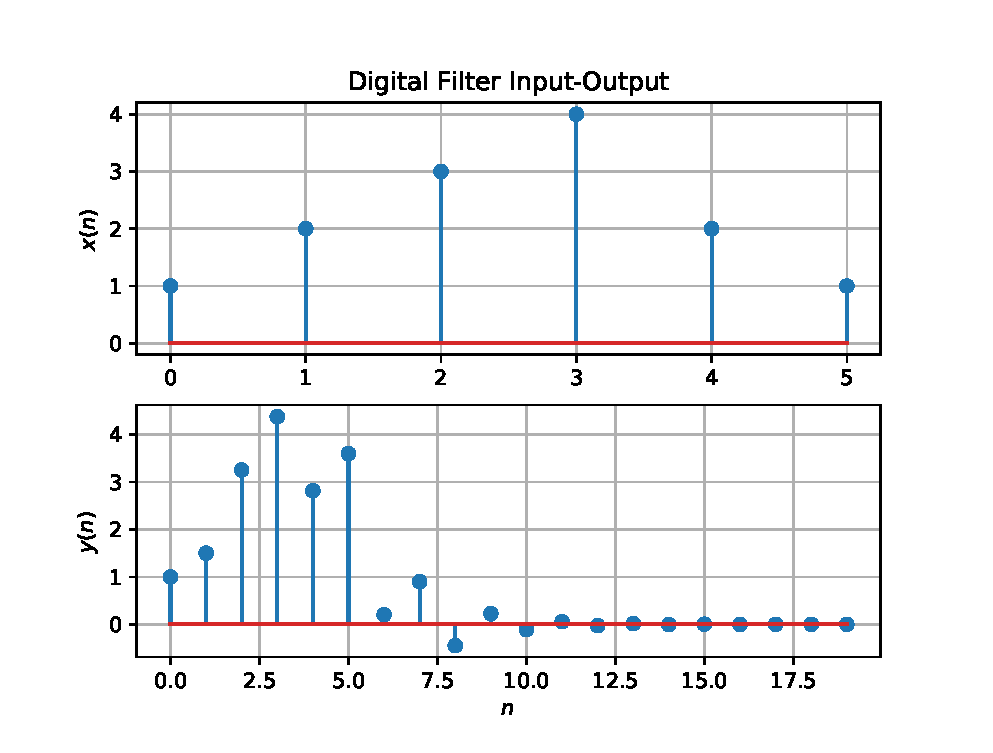
\includegraphics[width=\columnwidth]{./figs/xnyn}
\end{center}
\captionof{figure}{}
\label{fig:xnyn}	
\end{figure}


From equation \eqref{eq:iir_filter}, putting $n=0$ and $n=1$
\begin{align}
{y(0) = x(0)},
\\
{y(1) = \frac{-1}{2}y(0) + x(1)}
\end{align}
as the length of $x(n)$ is 6,
\item Repeat the above exercise with C code.
\\
Download the codes for this exercise from 
\begin{lstlisting}
https://github.com/kn-vardhan/EE3900/tree/main/Assignment_1/codes
\end{lstlisting}

\end{enumerate}
\section{$Z$-transform}
\begin{enumerate}[label=\thesection.\arabic*]
\item The $Z$-transform of $x(n)$ is defined as
%
\begin{equation}
\label{eq:z_trans}
X(z)={\mathcal {Z}}\{x(n)\}=\sum _{n=-\infty }^{\infty }x(n)z^{-n}
\end{equation}
%
Show that
\begin{equation}
\label{eq:shift1}
{\mathcal {Z}}\{x(n-1)\} = z^{-1}X(z)
\end{equation}
and find
\begin{equation}
	{\mathcal {Z}}\{x(n-k)\} 
\end{equation}
\solution From \eqref{eq:z_trans},
\begin{align}
{\mathcal {Z}}\{x(n-k)\} &=\sum _{n=-\infty }^{\infty }x(n-1)z^{-n}
\\
&=\sum _{n=-\infty }^{\infty }x(n)z^{-n-1} = z^{-1}\sum _{n=-\infty }^{\infty }x(n)z^{-n}
\end{align}
resulting in \eqref{eq:shift1}. Similarly, it can be shown that
%
\begin{equation}
\label{eq:z_trans_shift}
	{\mathcal {Z}}\{x(n-k)\} = z^{-k}X(z)
\end{equation}
\item Obtain $X(z)$ for $x(n)$ defined in problem 3.1
\\
\solution
\begin{align}
X(z) = \sum _{n=0 }^{5}x(n)z^{-n}
\end{align}
\begin{align}
X(z) = 1 + 2z^{-1} + 3z^{-2} + 4z^{-3} + 2z^{-4} + z^{-5}
\end{align}

\item Find
%
\begin{equation}
H(z) = \frac{Y(z)}{X(z)}
\end{equation}
%
from  \eqref{eq:iir_filter} assuming that the $Z$-transform is a linear operation.
\\
\solution  Applying \eqref{eq:z_trans_shift} in \eqref{eq:iir_filter},
\begin{align}
Y(z) + \frac{1}{2}z^{-1}Y(z) &= X(z)+z^{-2}X(z)
\\
\implies \frac{Y(z)}{X(z)} &= \frac{1 + z^{-2}}{1 + \frac{1}{2}z^{-1}}
\label{eq:freq_resp}
\end{align}
%
\item Find the Z transform of 
\begin{equation}
\delta(n)
=
\begin{cases}
1 & n = 0
\\
0 & \text{otherwise}
\end{cases}
\end{equation}
and show that the $Z$-transform of
\begin{equation}
\label{eq:unit_step}
u(n)
=
\begin{cases}
1 & n \ge 0
\\
0 & \text{otherwise}
\end{cases}
\end{equation}
is
\begin{equation}
U(z) = \frac{1}{1-z^{-1}}, \quad \abs{z} > 1
\end{equation}
\solution It is easy to show that
\begin{equation}
\delta(n) \ztrans 1
\end{equation}
and from \eqref{eq:unit_step},
\begin{align}
U(z) &= \sum _{n= 0}^{\infty}z^{-n}
\\
&=\frac{1}{1-z^{-1}}, \quad \abs{z} > 1
\end{align}
using the fomula for the sum of an infinite geometric progression.
%
\item Show that 
\begin{equation}
\label{eq:anun}
a^nu(n) \ztrans \frac{1}{1-az^{-1}} \quad \abs{z} > \abs{a}
\end{equation}
\solution Applying \eqref{eq:z_trans}
\begin{equation}
a^nU(z) = \sum _{n= 0}^{\infty}a^n u(n) z^{-n}
\end{equation}
and from (4.14), if $\abs{a} < \abs{z}$ 
\begin{equation}
a^nu(n) \ztrans \frac{1}{1-az^{-1}} \quad \abs{z} > \abs{a}
\end{equation}
%
\item 
Let
\begin{equation}
H\brak{e^{\j \omega}} = H\brak{z = e^{\j \omega}}.
\end{equation}
Plot $\abs{H\brak{e^{\j \omega}}}$.  Comment.  $H(e^{\j \omega})$ is
known as the {\em Discret Time Fourier Transform} (DTFT) of $x(n)$.
\\
{\textbf{Comment:}} The DTFT of $x(n)$ is a Fourier Analysis that is applicable to a sequcence of values. This produces a periodic function of a frequency variable. Here in $\abs{H(e^{\j \omega})}$, when the graph is plotted (Fig. \ref{fig:dtft}\:). 
\\
\solution The following code plots Fig. \ref{fig:dtft}.
\begin{lstlisting}
wget https://raw.githubusercontent.com/gadepall/EE1310/master/filter/codes/dtft.py
\end{lstlisting}
\begin{figure}[!ht]
\centering
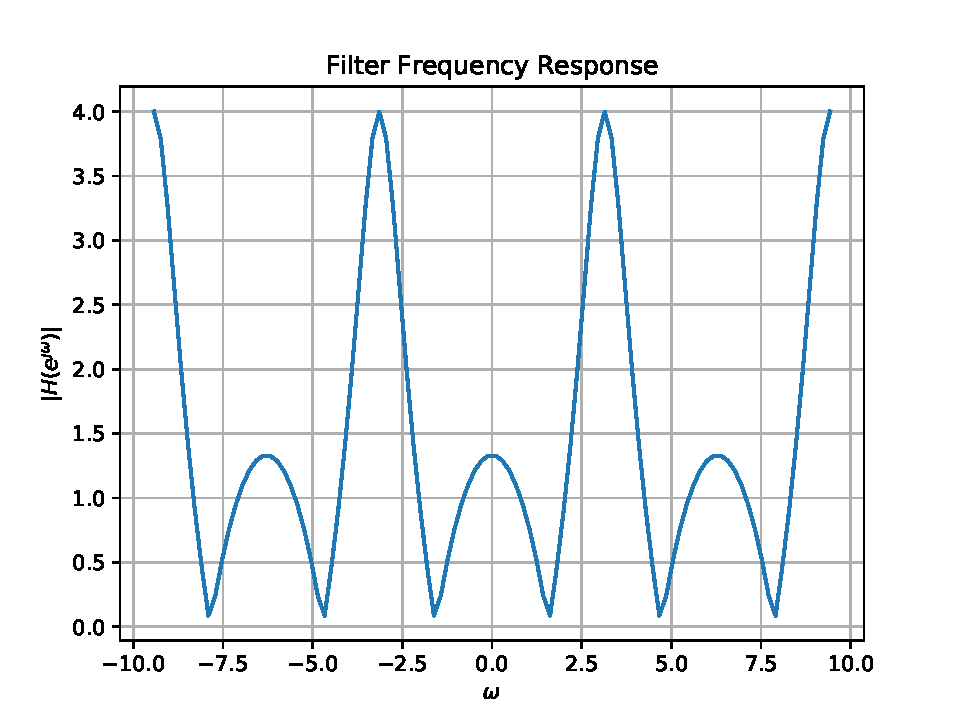
\includegraphics[width=\columnwidth]{./figs/dtft}
\caption{$\abs{H\brak{e^{\j\omega}}}$}
\label{fig:dtft}
\end{figure}
A function $f:A \rightarrow B$ is said to be periodic with a period $T$ if,
\begin{align}
f(t+T) = f(t)\:\: \forall \:t \in A
\end{align}
Now, for the fucntion $\abs{H(e^{j\omega})}$, it can be written as
\begin{align}
	\left|H\brak{e^{\j\omega}}\right| &= \left|\frac{1 + e^{-2\j\omega}}{1 + \frac{1}{2}e^{-\j\omega}}\right| \\
									  &= \sqrt{\frac{\brak{1 + \cos{2\omega}}^2 + \brak{\sin{2\omega}}^2}{\brak{1 + \frac{1}{2}\cos{\omega}}^2 + \brak{\frac{1}{2}\sin{\omega}}^2}}\\
									  &= \sqrt{\frac{2\brak{1 + \cos{2\omega}}}{\frac{5}{4} + \cos{\omega}}} \\
									  &= \sqrt{\frac{2\brak{2\cos^2{\omega}}}{\frac{5}{4} + \cos{\omega}}} \\
									  &= \frac{4|\cos{\omega}|}{\sqrt{5 + 4\cos{\omega}}}
\end{align}
Therefore, the period of $\abs{H(e^{j\omega})} = 2\pi$.
\\
\item Express $h(n)$ in terms of $H(e^{j\omega})$
\\
\solution We have,
\begin{align}
	H(e^{\j\omega}) &= \sum_{k = -\infty}^{\infty}h(k)e^{-\j\omega k}
\end{align}
However,
\begin{align}
	\int_{-\pi}^{\pi}e^{\j\omega(n - k)}d\omega =
	\begin{cases}
		2\pi & n = k \\
		0 & \textrm{otherwise}
	\end{cases}
\end{align}
and so,
\begin{align}
	&\frac{1}{2\pi}\int_{-\pi}^{\pi}H(e^{\j\omega})e^{j\omega n}d\omega \\
	&= \frac{1}{2\pi}\sum_{k = -\infty}^{\infty}\int_{-\pi}^{\pi}h(k)e^{\j\omega(n - k)}d\omega \\
	&= \frac{1}{2\pi}2\pi h(n) = h(n)
\end{align}
which is known as the Inverse Discrete Fourier Transform. Thus,
\begin{align}
	h(n) &= \frac{1}{2\pi}\int_{-\pi}^{\pi}H(e^{\j\omega})e^{\j\omega n}d\omega \\
		 &= \frac{1}{2\pi}\int_{-\pi}^{\pi}\frac{1 + e^{-2\j\omega}}{1 + \frac{1}{2}e^{-\j\omega}}e^{\j\omega n}d\omega
	\label{eq:idtft}
\end{align}
\end{enumerate}
\section{Impulse Response}
\begin{enumerate}[label=\thesection.\arabic*]
\item Using long division, find
\begin{align}
h(n), \quad n < 5
\end{align}
for H(z) in \eqref{eq:freq_resp}.
\\
\solution For long division, substitute $x := z^{-1}$
\polylongdiv{x^2 + 1}{1 + \frac{1}{2}x}
\\
Therefore,
\begin{align}
	H(z) &=  2z^{-1} - 4 + \frac{5}{1 + \frac{1}{2}z^{-1}} \\
		 &= 2z^{-1} - 4 + 5\sum_{n = 0}^{\infty}\brak{-\frac{1}{2}}^nz^{-n} \\
		 &= 1 - \frac{1}{2}z^{-1} + 5\sum_{n = 2}^{\infty}\brak{-\frac{1}{2}}^nz^{-n} \\
		 &= \sum_{n = 0}^{\infty}\brak{-\frac{1}{2}}^nz^{-n} + 4\sum_{n = 2}^{\infty}\brak{-\frac{1}{2}}^nz^{-n} \\
		 &= \sum_{n = -\infty}^{\infty}u(n)\brak{-\frac{1}{2}}^nz^{-n} + \nonumber \\
		 &\sum_{n = -\infty}^{\infty}u(n - 2)\brak{-\frac{1}{2}}^{n - 2}z^{-n}
\end{align}
Now, from \eqref{eq:z_trans}, we get
\begin{align}
	h(n) = \brak{-\frac{1}{2}}^{n}u(n) + \brak{-\frac{1}{2}}^{n-2}u(n-2)
\end{align}
\item \label{prob:impulse_resp}
Find an expression for $h(n)$ using $H(z)$, given that 
%in Problem \ref{eq:ztransab} and \eqref{eq:anun}, given that
\begin{equation}
\label{eq:impulse_resp}
h(n) \ztrans H(z)
\end{equation}
and there is a one to one relationship between $h(n)$ and $H(z)$. $h(n)$ is known as the {\em impulse response} of the
system defined by \eqref{eq:iir_filter}.
\\
\solution From \eqref{eq:freq_resp},
\begin{align}
H(z) &= \frac{1}{1 + \frac{1}{2}z^{-1}} + \frac{ z^{-2}}{1 + \frac{1}{2}z^{-1}}
\\
\implies h(n) &= \brak{-\frac{1}{2}}^{n}u(n) + \brak{-\frac{1}{2}}^{n-2}u(n-2)
\end{align}
using \eqref{eq:anun} and \eqref{eq:z_trans_shift}.
\item Sketch $h(n)$. Is it bounded? Justify theoritically. 
\\
\solution Yes, $h(n)$ is bounded as well as converges to $0$ when $n$ approaches to $\infty$.\\
The following code plots Fig. \ref{fig:hn}.
\begin{lstlisting}
wget https://raw.githubusercontent.com/gadepall/EE1310/master/filter/codes/hn.py
\end{lstlisting}
\begin{figure}[!ht]
\centering
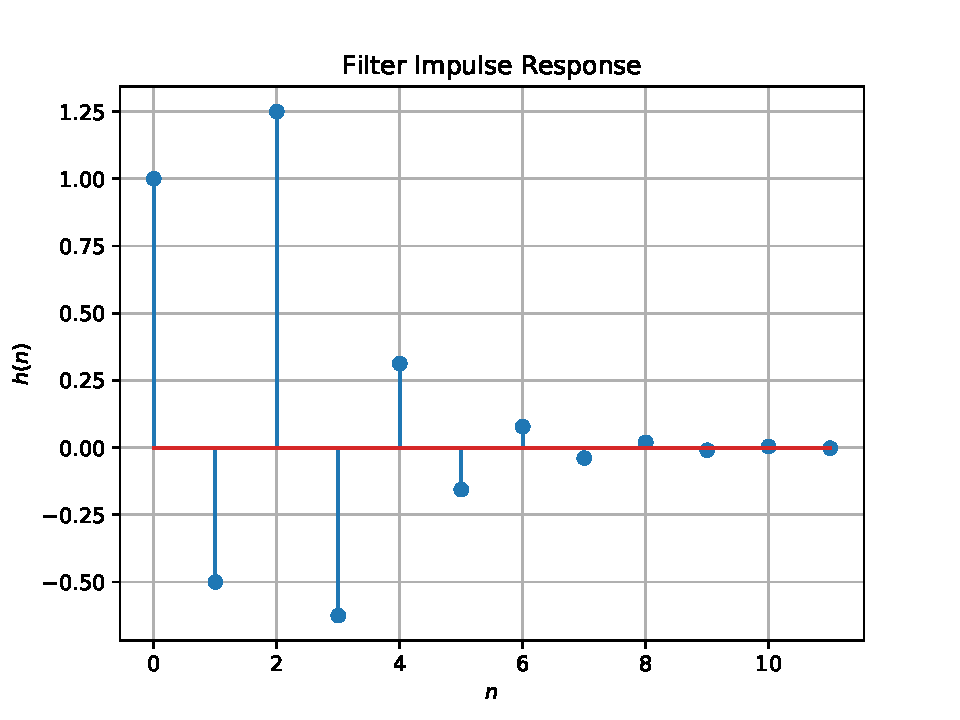
\includegraphics[width=\columnwidth]{./figs/hn}
\caption{$h(n)$ as the inverse of $H(z)$}
\label{fig:hn}
\end{figure}
For large values of $n$, we have $u(n) \rightarrow 1$\\
Therefore,
\begin{align}
h(n) &= \brak{-\frac{1}{2}}^n + \brak{-\frac{1}{2}}^{n - 2} \\
		 &= \brak{-\frac{1}{2}}^{n}\brak{4 + 1} = 5\brak{-\frac{1}{2}}^n \\
		 &\implies \left|\frac{h(n + 1)}{h(n)}\right| = \frac{1}{2}
\end{align}
\item Convergent? Justify using ratio test
\\
\solution From the above result, we have
\begin{align} 
\left|\frac{h(n + 1)}{h(n)}\right| = \frac{1}{2}
\end{align}
Therefore, we have,
\begin{align}
\lim_{n \to \infty}\left|\frac{h(n + 1)}{h(n)}\right| = \frac{1}{2} < 1
\end{align}
We can see that limit $<$ 1, therefore, $h(n)$ is convergent.
\item The system with $h(n)$ is defined to be stable if
\begin{equation}
\sum_{n=-\infty}^{\infty}h(n) < \infty
\end{equation}
Is the system defined by \eqref{eq:iir_filter} stable for the impulse response in \eqref{eq:impulse_resp}?
%
\\
\solution We have,
\begin{align}
	\sum_{n = -\infty}^{\infty}h\brak{n} &= \sum_{n = -\infty}^{\infty}
	\brak{-\frac{1}{2}}^nu\brak{n} + \brak{-\frac{1}{2}}^{n - 2}u\brak{n - 2} \\
										 &= 2\brak{\frac{1}{1 + \frac{1}{2}}} = \frac{4}{3}
\end{align}
Therefore, we can see that the given system with $h(n)$ is stable for the impulse response \eqref{eq:impulse_resp}.
\item Verify the above result using a python code.
\\
\item 
Compute and sketch $h(n)$ using 
\begin{equation}
\label{eq:iir_filter_h}
h(n) + \frac{1}{2}h(n-1) = \delta(n) + \delta(n-2), 
\end{equation}
%
This is the definition of $h(n)$.
\\
\solution The following code plots Fig. \ref{fig:hndef}. Note that this is the same as Fig. 
\ref{fig:hn}. 
%
\begin{lstlisting}
wget https://raw.githubusercontent.com/gadepall/EE1310/master/filter/codes/hndef.py
\end{lstlisting}
\begin{figure}[!ht]
\centering
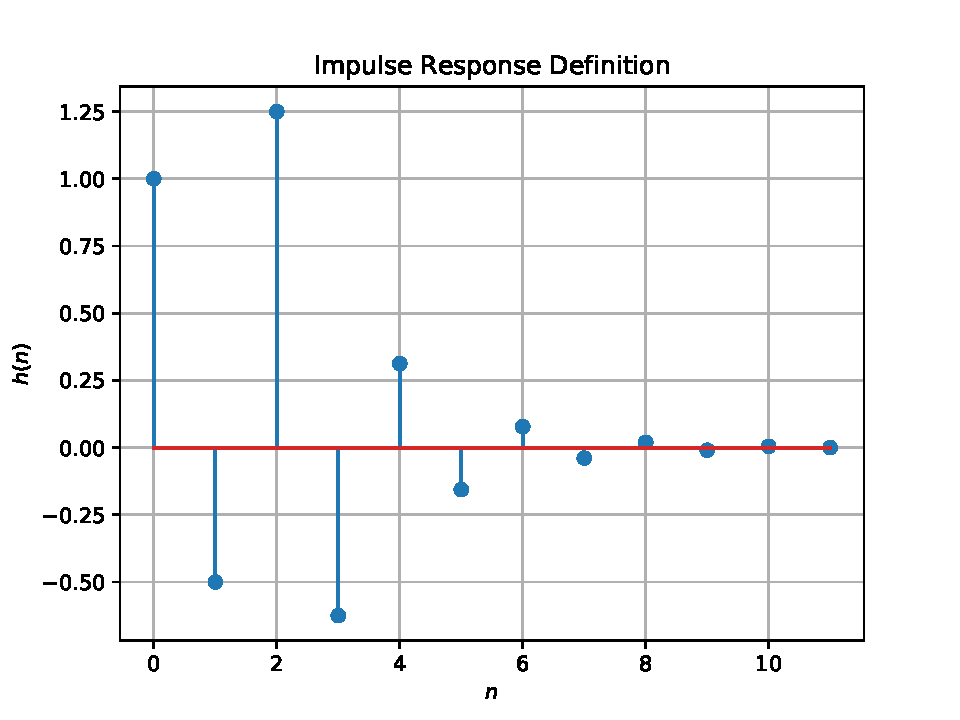
\includegraphics[width=\columnwidth]{./figs/hndef}
\caption{$h(n)$ from the definition}
\label{fig:hndef}
\end{figure}
%
\item Compute 
%
\begin{equation}
\label{eq:convolution}
y(n) = x(n)*h(n) = \sum_{n=-\infty}^{\infty}x(k)h(n-k)
\end{equation}
%
Comment. 
\\ The operation in \eqref{eq:convolution} is known as
{\em convolution}.
%
\\
\solution The following code plots Fig. \ref{fig:ynconv}. Note that this is the same as 
$y(n)$ in  Fig. 
\ref{fig:xnyn}. 
%
\begin{lstlisting}
wget https://raw.githubusercontent.com/gadepall/EE1310/master/filter/codes/ynconv.py
\end{lstlisting}
\begin{figure}[!ht]
\centering
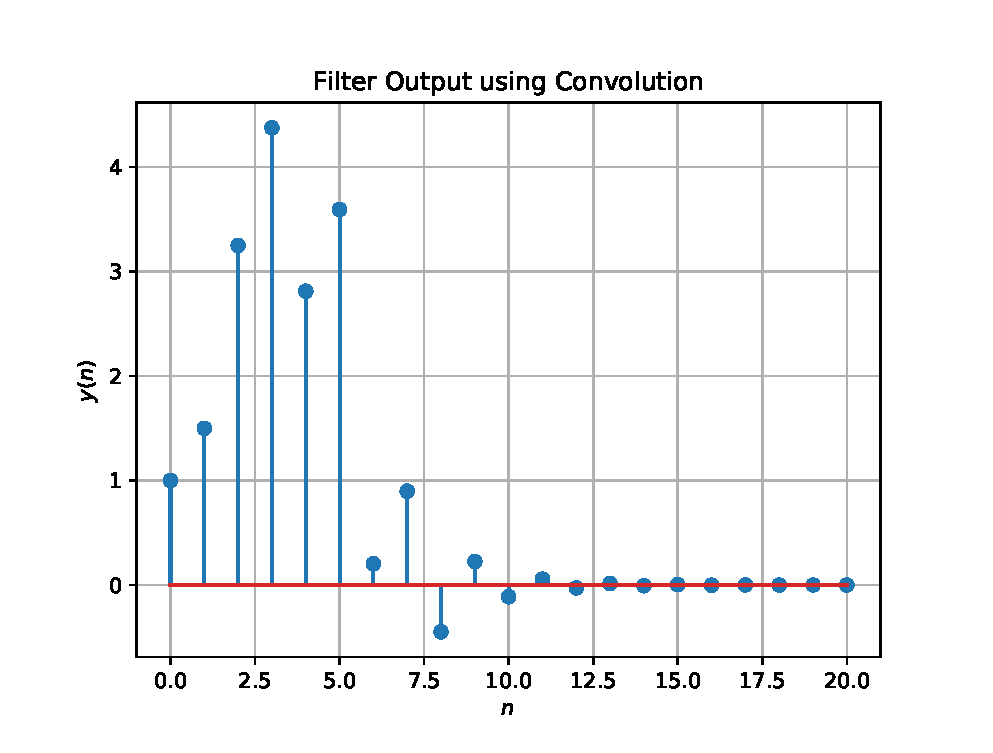
\includegraphics[width=\columnwidth]{./figs/ynconv}
\caption{$y(n)$ from the definition of convolution}
\label{fig:ynconv}
\end{figure}
\item Express the above convolution using a Toeplitz matrix.
\\
\solution 
\\The Toeplitz matrices for convolution are,
\begin{align}
	\mtx{y} &= \mtx{x} \circledast \mtx{h}\\
	\mtx{y} &= 
	\begin{pmatrix}
		h_1 & 0 & . & . & . & 0 \\
		h_2 & h_1 & . & . & . & 0 \\
		h_3 & h_2 & h_1 & . & . & 0 \\
		. & . & . & . & . & . \\
		0 & . & . & h_3 & h_2 & h_1 \\
		0 & . & . & . & h_2 & h_1 \\
		0 & . & . & . & 0 & h_1
	\end{pmatrix}
	\begin{pmatrix}
		x_1 \\ x_2 \\ \vdots \\ x_n
	\end{pmatrix}
\end{align}
\item Show that
\begin{equation}
y(n) =  \sum_{n=-\infty}^{\infty}x(n-k)h(k)
\end{equation}
\solution 
From \eqref{eq:convolution}, we substitute $k := n - k$ to get
\begin{align}
y\brak{n} &= \sum_{k=-\infty}^{\infty}x\brak{k}h\brak{n - k} \\
		  &= \sum_{n - k=-\infty}^{\infty}x\brak{n - k}h\brak{k} \\
		  &= \sum_{k=-\infty}^{\infty}x\brak{n - k}h\brak{k}
\end{align}
\end{enumerate}

%
\section{DFT and FFT}
\begin{enumerate}[label=\thesection.\arabic*]
\item
Compute
\begin{equation}
X(k) \define \sum _{n=0}^{N-1}x(n) e^{-\j2\pi kn/N}, \quad k = 0,1,\dots, N-1
\end{equation}
and $H(k)$ using $h(n)$.
\item Compute 
\begin{equation}
Y(k) = X(k)H(k)
\label{eq:fp}
\end{equation}
\item Compute
\begin{equation}
 y\brak{n}={\frac {1}{N}}\sum _{k=0}^{N-1}Y\brak{k}\cdot e^{\j 2\pi kn/N},\quad n = 0,1,\dots, N-1
 \label{eq:inv-ft}
\end{equation}
\\
\solution The following code plots Fig. \ref{fig:ynconv}. Note that this is the same as 
$y(n)$ in  Fig. 
\ref{fig:xnyn}. 
%
\begin{lstlisting}
wget https://raw.githubusercontent.com/gadepall/EE1310/master/filter/codes/yndft.py
\end{lstlisting}
\begin{figure}[!ht]
\centering
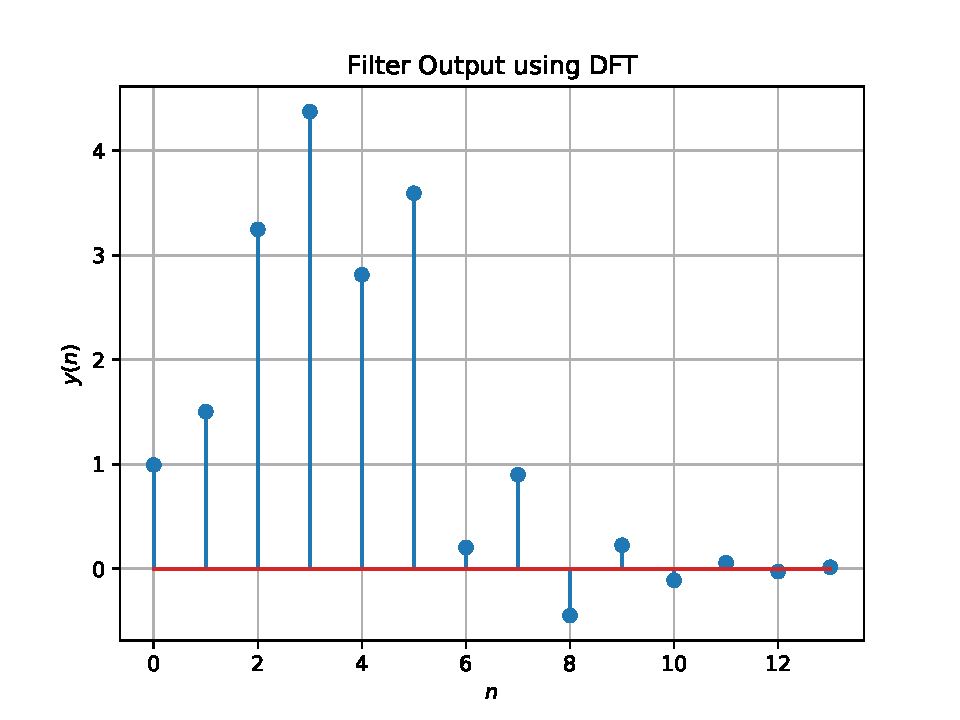
\includegraphics[width=\columnwidth]{./figs/yndft}
\caption{$y(n)$ from the DFT}
\label{fig:yndft}
\end{figure}

\item Repeat the previous exercise by computing $X(k), H(k)$ and $y(n)$ through FFT and 
IFFT.
\solution The python codes for the following can be downloaded from
\begin{lstlisting}
wget https://raw.githubusercontent.com/kn-vardhan/EE3900-Digital-Signal-Processing/main/Assignment_1/codes/fft-fft.py
\end{lstlisting}
and execute it using
\begin{lstlisting}
python3 fft-ifft.py
\end{lstlisting}
Observe that Fig. \eqref{fig:y-n-fft} is the same as $y(n)$ in Fig. \eqref{fig:xnyn}.
\begin{figure}
	\centering
	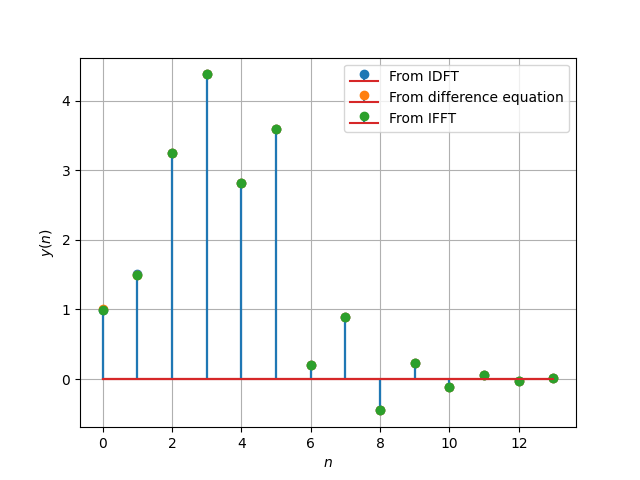
\includegraphics[width=\columnwidth]{figs/fft-ifft.png}
	\caption{$y(n)$ using FFT and IFFT}
	\label{fig:y-n-fft}
\end{figure}
\item Wherever possible, express all the above equations as matrix equations.
\\
\solution 
\\We use the DFT Matrix, where $\omega = e^{-\frac{j2k\pi}{N}}$, which is given by
\begin{align}
	\mtx{W} = 
	\begin{pmatrix}
		\omega^0 & \omega^0 & \ldots & \omega^0 \\
		\omega^0 & \omega^1 & \ldots & \omega^{N - 1} \\
		\vdots & \vdots & \ddots & \vdots \\
		\omega^0 & \omega^{N - 1} & \ldots & \omega^{(N -1)(N - 1)}
	\end{pmatrix}
\end{align}
i.e. $W_{jk} = \omega^{jk}$, $0 \leq j, k < N$. Hence, we can write any DFT equation as
\begin{align}
	\mtx{X} = \mtx{W}\mtx{x} = \mtx{x}\mtx{W}
\end{align}
\noindent where
\begin{align}
	\mtx{x} = 
	\begin{pmatrix}
		x(0) \\ x(1) \\ \vdots \\ x(n - 1)
	\end{pmatrix}
\end{align}
Using $\eqref{eq:inv-ft}$, the inverse Fourier Transform is given by
\begin{align}
	\mtx{x} = \mathcal{F}^{-1}\brak{\mtx{X}} = \mtx{W}^{-1}\mtx{X} &= 
	\frac{1}{N}\mtx{W^{H}}\mtx{X} = \frac{1}{N}\mtx{X}\mtx{W^{H}} \\ 
	\implies \mtx{W}^{-1} &= \frac{1}{N}\mtx{W^{H}}
\end{align}
\noindent where $H$ denotes hermitian operator. We can rewrite \eqref{eq:fp} using the
element-wise multiplication operator as
\begin{align}
	\mtx{Y} = \mtx{H}\cdot\mtx{X} = \brak{\mtx{W}\mtx{h}}\cdot\brak{\mtx{W}\mtx{x}}
\end{align}
The plot of $y(n)$ using the DFT matrix in Fig. \ref{fig:yn-mtx} is the same as $y(n)$ in 
Fig. \eqref{fig:xnyn}.
\begin{figure}[!htb]
	\centering
	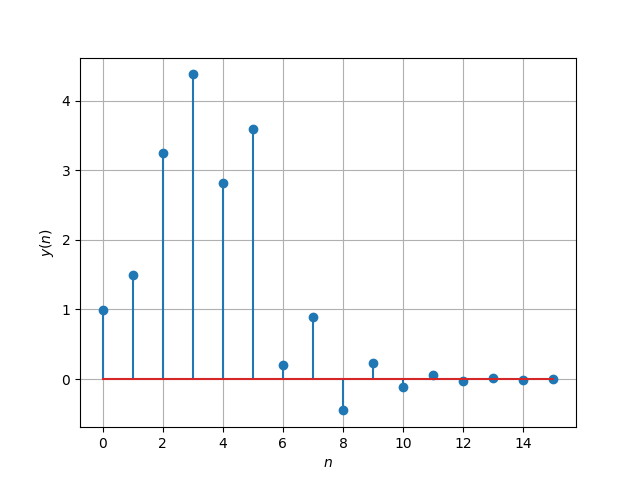
\includegraphics[width=\columnwidth]{figs/6_5.png}
	\caption{$y(n)$ using the DFT matrix}
	\label{fig:yn-mtx}
\end{figure}
\item Verify the above equations by generating the DFT matrix in python.
\\
\solution The code for the following question can be downloaded from
\begin{lstlisting}
$ wget https://raw.githubusercontent.com/kn-vardhan/EE3900-Digital-Signal-Processing/main/Assignment_1/codes/6_6.py
\end{lstlisting}
and can be executed using the command
\begin{lstlisting}
$ python3 6_6.py
\end{lstlisting}
The plot is shown in Fig. \eqref{fig:yn-own}
\begin{figure}
	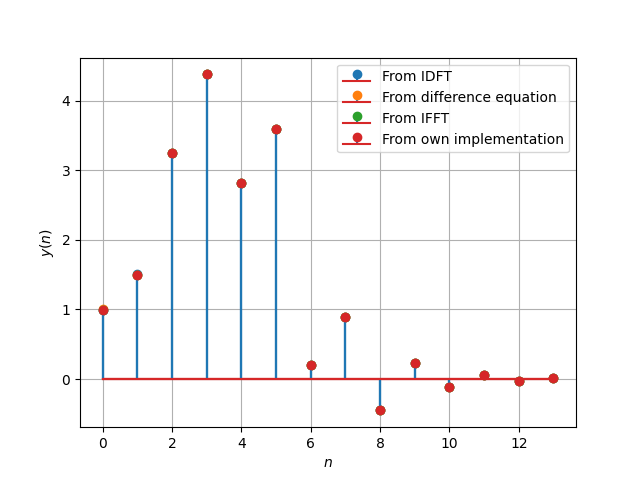
\includegraphics[width=\columnwidth]{figs/6_6.png}
	\caption{Own implementation of FFT and IFFT}
	\label{fig:yn-own}
\end{figure}
%\begin{lstlisting}
%$ wget https://raw.githubusercontent.com/goats-9/ee3900-assignments/main/Assignment_01/codes/6_5.py
%\end{lstlisting}
%\item Find the time complexities of computing $y(n)$ using the FFT/IFFT and convolution.
\end{enumerate}
\section{FFT}
\begin{enumerate}[label=\thesection.\arabic*.,ref=\thesection.\theenumi]
\numberwithin{equation}{section}
    \item The DFT of $x(n)$ is given by
    \begin{align}
        X(k) \triangleq \sum_{n=0}^{N-1} x(n) e^{-j 2 \pi k n / N}, \quad k=0,1, \ldots, N-1
    \end{align}
\item Let 
	\begin{align}
W_{N} = e^{-j2\pi/N} 
	\end{align}
		Then the $N$-point {\em DFT matrix} is defined as 
	\begin{align}
		\vec{F}_{N} = \sbrak{W_{N}^{mn}}, \quad 0 \le m,n \le N-1 
	\end{align}
	where $W_{N}^{mn}$ are the elements of $\vec{F}_{N}$.
\newpage
\item Let 
	\begin{align}
		\vec{I}_4 = \myvec{\vec{e}_4^{1} &\vec{e}_4^{2} &\vec{e}_4^{3} &\vec{e}_4^{4} }
	\end{align}
		be the $4\times 4$ identity matrix.  Then the 4 point {\em DFT permutation matrix} is defined as 
	\begin{align}
		\vec{P}_4 = \myvec{\vec{e}_4^{1} &\vec{e}_4^{3} &\vec{e}_4^{2} &\vec{e}_4^{4} }
	\end{align}
\item The 4 point {\em DFT diagonal matrix} is defined as 
	\begin{align}
		\vec{D}_4 = diag\myvec{W_{8}^{0} & W_{8}^{1} & W_{8}^{2} & W_{8}^{3}}
	\end{align}
\item Show that 
\begin{equation}
    W_{N}^{2}=W_{N/2}
	\label{eq:n-2}
\end{equation}
\solution We can check that
\begin{align}
	W_N^2 = \brak{e^{-\frac{\j2\pi}{N}}}^2 = e^{-\frac{\j2\pi}{N/2}} = W_{N/2}
\end{align}
\item Show that 
\begin{equation}
	\vec{F}_{4}=
\begin{bmatrix}
	\vec{I}_{2} & \vec{D}_{2} \\
\vec{I}_{2} & -\vec{D}_{2}
\end{bmatrix}
\begin{bmatrix}
\vec{F}_{2} & 0 \\
0 & \vec{F}_{2}
\end{bmatrix}
\vec{P}_{4}
\label{eq:fft-recurrence}
\end{equation}

\solution Observe that for $n \in \mathbb{N}$, $W_4^{4n} = 1$ and $W_4^{4n + 2} = -1$. Using \eqref{eq:n-2},
\begin{align}
	\vec{D}_2\vec{F}_2 &= \mybvec{\w{4}{0} & 0 \\ 0 & \w{4}{1}}\mybvec{\w{2}{0} & \w{2}{0} \\ \w{2}{0} & \w{2}{1}} \\
					   &= \mybvec{\w{4}{0} & 0 \\ 0 & \w{4}{1}}\mybvec{\w{4}{0} & \w{4}{0} \\ \w{4}{0} & \w{4}{2}} \\
					   &= \mybvec{\w{4}{0} & \w{4}{0} \\ \w{4}{1} & \w{4}{3}} \label{eq:fft-df1} \\
	\implies -\vec{D}_2\vec{F}_2 &= \mybvec{\w{4}{2} & \w{4}{6} \\ \w{4}{3} & \w{4}{9}} \label{eq:fft-df2}
\end{align}
and
\begin{align}
	\vec{F}_2 &= \myvec{\w{2}{0} & \w{2}{0} \\ \w{2}{0} & \w{2}{1}} \\
			  &= \myvec{\w{4}{0} & \w{4}{0} \\ \w{4}{0} & \w{4}{2}}
\end{align}
Hence,
\begin{align}
	\vec{W}_4 &= \myvec{\w{4}{0} & \w{4}{0} & \w{4}{0} & \w{4}{0} \\
		\w{4}{0} & \w{4}{2} & \w{4}{1} & \w{4}{3} \\
		\w{4}{0} & \w{4}{4} & \w{4}{2} & \w{4}{6} \\
		\w{4}{0} & \w{4}{6} & \w{4}{3} & \w{4}{9} 
	} \label{eq:fft-permutation} \\
	&= \mybvec{\vec{I}_2\vec{F}_2 & \vec{D}_2{F}_2 \\ \vec{I}_2\vec{F}_2 & -\vec{D}_2{F}_2} \\
	&= \mybvec{\vec{I}_2 & \vec{D}_2 \\ \vec{I}_2 & \vec{D}_2}\mybvec{\vec{F}_2 & 0 \\ 0 & \vec{F}_2}
	\label{eq:ifd}
\end{align}
Multiplying \eqref{eq:ifd} by $\vec{P}_4$ on both sides, and noting that $\vec{W}_4\vec{P}_4 = \vec{F}_4$ gives us \eqref{eq:fft-recurrence}.

\end{enumerate}

\end{document}

